%%%%%%%%%%%%%%%%%%%%%%%%%%%%%%%%%%%%%%%%%%%%%%%%%%%%%%%%%%%%%%%%%%%%%%%%%%%%%%%%%%
%% MS: In Focus comment paper for Journal of Animal Ecology.
%% Draft
%% April 2016
%% Revised version: 
%% Original version wordcount: 1688 words.
%%%%%%%%%%%%%%%%%%%%%%%%%%%%%%%%%%%%%%%%%%%%%%%%%%%%%%%%%%%%%%%%%%%%%%%%%%%%%%%%%%
\documentclass[a4paper,12pt]{article}
\usepackage{comment}
\usepackage{jae}
\title{IN FOCUS \\ Natural history matters: how biological constraints shape diversified interactions in pollination networks}
\running{Forbidden interactions}

\author{Pedro Jordano$^{1}$}

\affiliations{
\item Integrative Ecology Group, Estaci\'on Biol\'ogica de Do\~nana, Consejo Superior de Investigaciones Cient\'ificas (EBD-CSIC), Avenida Americo Vespucio s\slash n, E--41092 Sevilla, Spain
}

\nwords{910}
\ntables{0}
\nfig{1}
\nref{7}

\corr{\url{jordano@ebd.csic.es}}
%---------------------------------------------------------------------------------
\begin{document}

\maketitle

%\begin{abstract}
  \noindent 
  IN FOCUS: Sazatornil, F.D., Moré, M., Benitez-Vieyra, S., Cocucci, A.A., Kitching, I.J., Schlumpberger, B.O., Oliveira, P.E., Sazima, M. \& Amorim, F.W. (2016) Beyond neutral and forbidden links: morphological matches and the assembly of mutualistic hawkmoth-plant networks. Journal of Animal Ecology, 00, 000–000. doi:10.1111\/1365-2656.12509 \\
  
  \textbf{Species-specific traits and life-history characteristics constrain the ways organisms interact in nature. For example, gape-limited predators are constrained in the sizes of prey they can handle and efficiently consume. When we consider the ubiquity of such constrains it is evident how hard it can be to be a generalist partner in ecological interactions: a free living animal or plant can't simply interact with every available partner it encounters. Some pairwise interactions among coexisting species simply do not occur; they are impossible to observe despite the fact that partners coexist in the same place. Sazatornil \textit{et al.} \citep{Sazatornil:2016} explore the nature of such constraints in the mutualisms among hawkmoths and the plants they pollinate. In this iconic interacion, used by Darwin and Wallace to vividly illustrate the power of natural selection in shaping evolutionary change, both pollinators and plants are sharply constrained in their interaction modes and outcomes. } \\
%\end{abstract}

\noindent \textbf{Keywords:} complex networks, forbidden links, long-tubed flowers, mutualism, pollination, Sphingidae

\newpage

%---------------------------------------------------------------------------------
Size-limited foragers show clear restrictions on the size of prey items they can efficiently handle. In the case of plant-pollinator interactions, size uncoupling between pollinator bodies and flower sizes or structure are specially relevant in filtering out a range of potential partners \citep{Cocucci:2009}. The idea, when applied to the bizarre flowers of some plants pollinated by sphingid moths (Lepidoptera: Sphingidae) (Fig. 1), was seminal in Darwinian evolutionary theory to support the potential of natural selection in shaping adaptations \citep{Arditti:2012}. Wallace \citep{Wallace:1867} in his book, \textit{Creation by law}, vividly uses the famous example of the Malagasy orchid and its sphingid pollinator to refute the arguments of the Duke of Argyll against natural selection and Darwinism:

\begin{spacing}{1.0}
	\begin{quotation}
	 "There is a Madagascar Orchis--the \textit{Angræcum sesquipedale}--with an immensely long and deep nectary. How did such an extraordinary organ come to be developed? Mr. Darwin's [[p. 475]] explanation is this. The pollen of this flower can only be removed by the proboscis of some very large moths trying to get at the nectar at the bottom of the vessel. The moths with the longest proboscis would do this most effectually; they would be rewarded for their long noses by getting the most nectar; whilst on the other hand, the flowers with the deepest nectaries would be the best fertilized by the largest moths preferring them. Consequently, the deepest nectaried Orchids and the longest nosed moths would each confer on the other a great advantage in the 'battle of life.' This would tend to their respective perpetuation and to the constant lengthening of nectar and noses."
	 \end{quotation}
 \end{spacing}
 
 Phenotypic fitting of corolla length and shape and the pollinators' feeding apparatus and body sizes are important because the better the fit, the better the consequences in terms of fitness outcomes for the interaction partners \citep{Nilsson:1988}. Yet the expectation of perfect trait matching across populations or communities is too simplistic \citep{Anderson:2010}: "arms races" as initially suggested by Darwin and Wallace are frequently asymmetric, originating pollinator shifts rather than tight phenotypic trait matching (Fig. 2). Extensive local variation in phenotypic mismatch exists in different plant-pollinator systems \citep[e.g., ][]{Cocucci:2009,Anderson:2010,More:2012}, with pollinator-mediated selection geographic mosaics of locally coevolved partners.

Recent work by Sazatornil \textit{et al.} \citep{Sazatornil:2016} provides evidences that the types of trait mismatching outlined in Fig. 2 limit the ranges of host plants for sphingid pollinators, and ultimately shape their complex plant-pollinator networks. By using a comparative analysis of five different hawkmoth/flower assemblages across four South American biotas (Atlantic rainforest and Cerrado in Brazil, Chaco montane dry woodland, and the ecotone between western Chaco woodland and Yungas montane rain forest in Argentina) they tested the contributions of phenotypic matching to explain observed patterns of moth-flower interactions. 

How are these moth-flower interactions assembled? Sazatornil \textit{et al.} \citep{Sazatornil:2016} first tested a neutral model, where interactions are independent of trait-matching. Under this hypothesis distribution parameters (mean and standard deviation) must be the same for both distributions. They further tested a Forbidden links hypothesis, where interactions occurred only if the hawkmoth proboscis length (HPL) is equal to or greater than the effective length of the flower (EFL). EFL is just the corolla tube length (as in Fig. 2 for long-tubed and salverform corollas) or the stamen protrusion length in brush-type and funnel-shape flowers (as in Fig. 1). Sazatornil \textit{et al.} further tested the morphological match hypothesis, where the probability of occurrence of an interaction depends on the frequency of possible pairwise differences between HPL and EFL, i.e., all possible pairwise HPL-EFL differences were weighted by their respective interaction frequency.

Th trait matching between HPL and EFL is crucial in this type of interaction and determines its outcome in terms of fitness for both partners. Nilsson \citep{Nilsson:1988} demonstrated experimentally that shortening the nectary tube of long-spurred corollas decreased both seed set and pollinia removal for \textit{Platanthera} orchids. Further experimental evidence has been provided for long-tongued nemestrinid flies pollinating long-tubed irises in South Africa, where increased mismatch decreases both plant fitness and the nectar extraction efficiency of the pollinators \citep{Pauw:2009}. Sazatornil \textit{et al.} extend those results to the scale of the whole moth-plant assemblage and demonstrate that trait matching successfully predicts the diversity of interactions recorded. Interestingly enough, the interaction patterns in two local assemblages from ecotone areas of the Chaco woodland-Yungas montane rain forest transition are better fitted by a neutral model where pairwise interactions are driven by probability of interspecific encounter. Yet Sazatornil \textit{et al.} did not include the morphological difference for parameter estimation when interactions were not recorded. Thus the test of the mismatch hypothesis implicitly includes forbidden links effects: a full mismatch of corolla tube/proboscis lengths actually means a forbidden link. Furthermore,  a fraction of unobserved interactions was likely caused by phenological uncoupling between flowering and hawkmoth activity phenophases \citep{BasJor:2014,Sazatornil:2016}. In any case the mismatch hypothesis somehow captures the fact that a fraction of the unobserved interactions in these hawkmoth/flower assemblages is due to extreme phenotypic mismatch, i.e., size-related forbidden links \citep{Sazatornil:2016}; also see \citep{VizentinBugoni:2014} for evidences with hummingbird-flower interactions. 

% Forbidden links background.
% Explain the biological basis of mismatch using Fig 2 and Arditti
Forbidden links represent a family of causes for not observing specific interactions when sampling diversified plant-animal interaction networks, and stem on biological causes deeply linked to the fascinating natural history details of these interactions \citep{BasJor:2014}. The raw material for phenotypic mismatches in the specific case of hawkmoth-flower interactions is the extreme variability of the two pivotal traits determining their outcomes: proboscis length and corolla/spur or nectary depth (Fig. 2) \citep{Cocucci:2009,Arditti:2012,Nilsson:1988,Miller:1997}. 

Sazatornil et al. approach would be most useful for proper tests of coevolutionary hypotheses in hawkmoth/flower assemblages (and plant-animal mutualisms in general): assessing match/mismatch patterns for every possible pairwise interaction among partners within complex webs of interaction where multiple life-history attributes may contribute biological reasons to expect forbidden links. The morphological match hypothesis is not the only mechanism to explain patterns of hawkmoth–plant interactions, where other life-history limitations may operate generating forbidden links, e.g., phenological mismatches (for example in the case of long-distance or elevational migratory hawkmoths), constraints from foraging for oviposition sites \citep{Alarcon:2008}, energetic constraints due to balances of nectar availability/foraging costs \citep{Borrell:2005}, etc.

%---------------------------------------------------------------------------------

\section*{Acknowledgments}

My work was funded by a Severo-Ochoa Excellence Grant (SEV2012-0262) from the Spanish Ministerio de Econom\'ia y Competitividad (MINECO), and RNM-5731 from the Junta de Andaluc\'ia. Andrea Cocucci generously provided material for Fig. 1 and insightful discussions on sphingids and long-tubed flowers.

\newpage

%---------------------------------------------------------------------------------
% Bibliography
% \bibliography{ms_infocus}
%%% Unnumbered Literature Cited

\begin{thebibliography}{10}

\bibitem{Sazatornil:2016}
Sazatornil, F.D., Moré, M., Benitez-Vieyra, S., Cocucci, A.A., Kitching, I.J., Schlumpberger, B.O., Oliveira, P.E., Sazima, M. \& Amorim, F.W. (2016) Beyond neutral and forbidden links: morphological matches and the assembly of mutualistic hawkmoth-plant networks. Journal of Animal Ecology, 00, 000–000.

\bibitem{Cocucci:2009}
Cocucci, A.A., Mor\'e, M. \& S\'ersic, A.N. (2009) Restricciones mec\'anicas en las interacciones planta-polinizador: estudio de casos en plantas polinizadas por esf\'ingidos. Interacciones planta---animal y la conservaci\'on de la biodiversidad (eds R. Medel, R. Zamora, M. Aizen \& R. Dirzo), pp. 43–59. CYTED, Madrid.

\bibitem{Arditti:2012}
Arditti, J., Elliott, J., Kitching, I.J. \& Wasserthal, L.T. (2012) “Good Heavens what insect can suck it”–Charles Darwin, \textit{Angraecum sesquipedale} and \textit{Xanthopan morganii praedicta}. Botanical Journal of the Linnean Society, 169, 403–432.

\bibitem{Wallace:1867}
Wallace, A.R. (1867) Creation by law. The Quarterly Journal of Science, 4, 471–488.

\bibitem{Nilsson:1988}
Nilsson, L.A. (1988) The evolution of flowers with deep corolla tubes. Nature, 334, 147–149.

\bibitem{Pauw:2009}
Pauw, A., Stofberg, J. \& Waterman, R.J. (2009) Flies and flowers in Darwin's race. Evolution, 63, 268–279.


\bibitem{VizentinBugoni:2014}
Vizentin-Bugoni, J., Maruyama, P.K. \& Sazima, M. (2014) Processes entangling interactions in communities: forbidden links are more important than abundance in a hummingbird-plant network. Proceedings of the Royal Society of London Series B-Biological Sciences, 281, 20132397.

\bibitem{Anderson:2010}
Anderson, B., Terblanche, J.S. \& Ellis, A.G. (2010) Predictable patterns of trait mismatches between interacting plants and insects. BMC Evolutionary Biology, 10, 204.

\bibitem{More:2012}
Moré, M., Amorim, F.W., Benitez-Vieyra, S., Medina, A.M., Sazima, M. \& Cocucci, A.A. (2012) Armament imbalances: match and mismatch in plant-pollinator traits of highly specialized long-spurred orchids (ed M. Heil). PLoS ONE, 7, e41878.

\bibitem{Miller:1997}
Miller, W.E. (1997) Diversity and evolution of tongue length in hawkmoths (Sphingidae). Journal of the Lepidopterists Society, 51, 9–31.

\bibitem{Alarcon:2008}
Alarcón, R., Davidowitz, G. \& Bronstein, J.L. (2008) Nectar usage in a southern Arizona hawkmoth community. Ecological Entomology, 33, 503–509.

\bibitem{Borrell:2005}
Borrell, B. (2005) Long tongues and loose niches: Evolution of euglossine bees and their nectar flowers. Biotropica, 37, 664–669.

\bibitem{BasJor:2014}
Bascompte, J. \& Jordano, P. (2014) Mutualistic Networks. Princeton University Press, Princeton, NJ.

\end{thebibliography}

%---------------------------------------------------------------------------------

\begin{flushright}
  \noindent 
  		\textbf{Pedro Jordano }\\
  		\begin{spacing}{1.0}
		\textit{Integrative Ecology Group, Estaci\'on Biol\'ogica de Do\~nana, \\ Consejo Superior de Investigaciones Cient\'ificas (EBD-CSIC), \\ Avenida Americo Vespucio s\slash n, \\ E--41092 Sevilla, Spain}
		\end{spacing}
\end{flushright}
\newpage

%---------------------------------------------------------------------------------
\section*{Figures}


\begin{figure}[h!]
  \caption{Morphological mismatches set important biological constraints for size-limited foragers, including e.g., predators, pollinators, and frugivores. In plant-animal mutualisms, a morphological mismatch between partners sets size limits that filter out a range of phenotypes that otherwise could eventually interact. Other reasons for forbidden links include, e.g., phenological differences \citep{BasJor:2014}. Thus, a number of the potential interactions that could take place in a given mutualistic assemblage simply cannot occur because of biological reasons: these are forbidden interactions. Photo: Andrea Cocucci. An sphingid moth, \textit{Agrius cingulata}, visiting a flower of \textit{Bauhinia mollis} (Fabaceae), Las Yungas, Argentina.}
  \label{Fig1}
  \begin{center}
    \includegraphics[width=14cm]{Fig1}
  \end{center}
\end{figure}

\begin{figure}[h!]
  \caption{The mechanistic basis of morphological mismatches in hawkmoth-flower interactions. Modified and redrawn from \citep{Arditti:2012}.}
  \label{Fig2}
  \begin{center}
    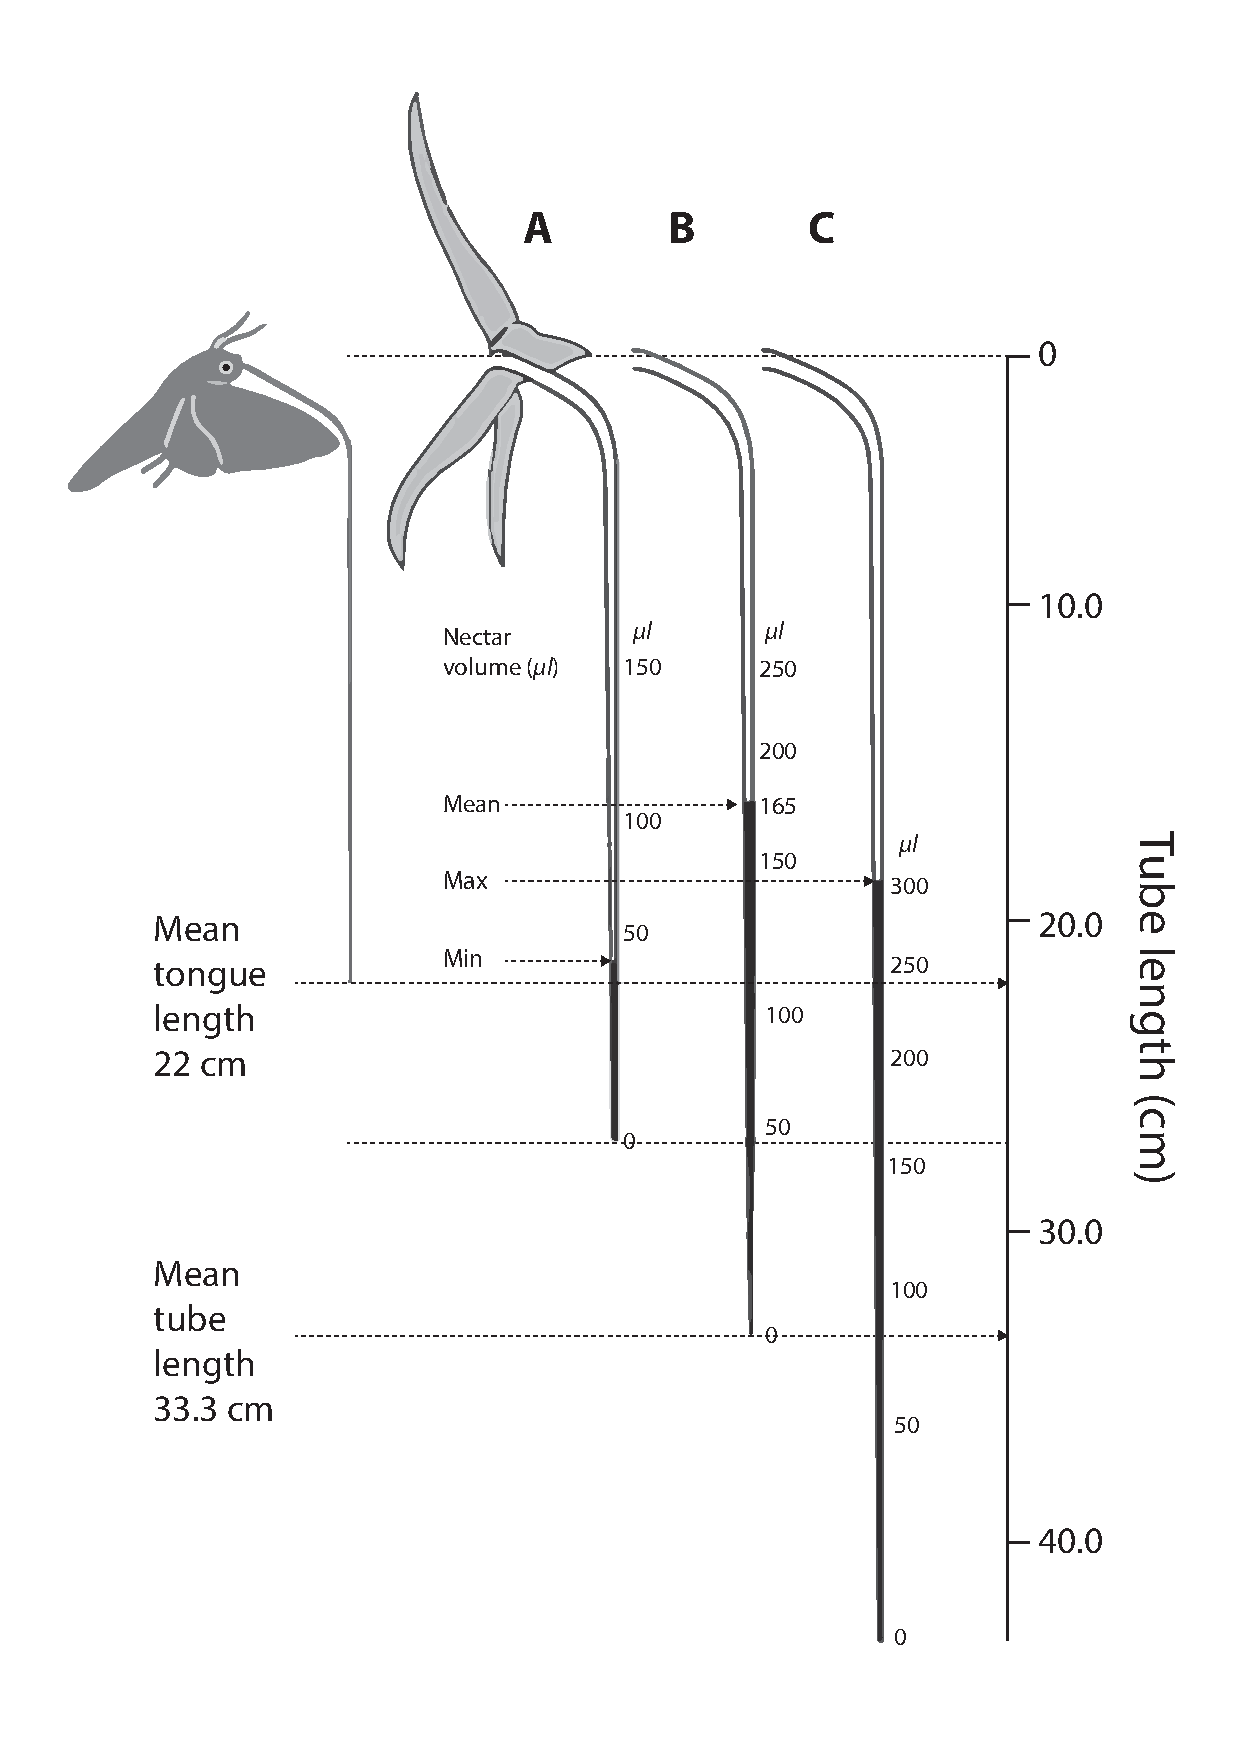
\includegraphics[width=14cm]{Fig2}
  \end{center}
\end{figure}
%---------------------------------------------------------------------------------
%%%%%%%%%%%%%%%%%%%%%%%%%%%%%%%%%%%%%%%%%%%%%%%%%%%%%%%%%%%%%%%%%%%%%%%%% MS NOTES
\begin{comment}
Arditti et al. Fig 11 legend:
Figure 11. Nectar: sugar content and height of column, proboscis length and coevolution. A, correlation between spur length and extracted nectar volume (modified from Wasserthal, 1997 by the removal of data about species other than Angraecum sesquipedale and the addition of the five lines of text at the base of the figure). B, correlation between height of nectar column and nectar volume measured by extraction and injection (modified from Wasserthal, 1997 by the addition of the two lines of text which start with ‘Mean’). C, comparison between Darwin’s ‘coevolution race’ and Wasserthal’s ‘pollinator shift’ models. In the ‘coevolution race’ model (A) the race is between increasing lengths of spurs and proboscises. The ‘pollination shift’ model (B) involves the recruitment by long-spurred angraecoid orchids of pollinators which are generalist feeders and have proboscises of different lengths. These pollinators are substituted gradually. When spurs enlarge beyond a certain length due to evolutionary pressure by the primary visitors flowers can be exploited (i.e. nectar can be taken from them) by illegitimate visitors with longer proboscises (*). This has been observed in interactions between Xanthopan morganii praedicta and Coelonia solani with Angraecum compactum. Increased selective pressure is exerted by the existence of moth species with long proboscises. Flowers become deceptive, but can still be pollinated when spurs become too long for the primary pollinator to reach the nectar. Pollination is impossible when the proboscis is longer than the spurs because the pollinaria are attached further from the base of the proboscis. When this happens the pollinaria are scratched away by the forelegs when the proboscis is rolled to a loose spiral. If the proboscis is shorter than the spur, transfer of the pollinaria is possible as long as the proboscis can get in contact with the sexual organs of the orchid. This occurs in other angrecoid orchids. Explanation of symbols: *, illegitimate visitor with a long proboscis which exploits flowers; black moth, orchid pollinator; grey moth, non-pollinating visitor; white moth, a moth incapable of pollinating an orchid (modified from Wasserthal, 1997 by moving and adding labels). D, correlation between position of fully inserted proboscis and time of insertion, stay and withdrawal (modified from Wasserthal, 1997 by the removal of data not pertaining to Angraecum sesquipedale). E, Nectar accessibility in Angraecum sesquipedale spurs. a, moth with an average spur length of 22 cm can obtain about 50 mL nectar from a spur of average length of 33.3 cm and an average nectar volume of 165 ml. b, a spur 43 cm long could offer nectar to a moth with a 22-cm-long proboscis only if it contains more than 240 mL solution. C, small volumes of nectar can be exploited if the spur is 27 cm long (Wasserthal, 1997).

\end{comment}
%%%%%%%%%%%%%%%%%%%%%%%%%%%%%%%%%%%%%%%%%%%%%%%%%%%%%%%%%%%%%%%%%%%%%%%%%%%%%%%%%%
\end{document}

